%% LyX 2.0.4 created this file.  For more info, see http://www.lyx.org/.
%% Do not edit unless you really know what you are doing.
\documentclass[11pt,oneside,english]{amsart}
\usepackage[T1]{fontenc}
\usepackage[latin9]{inputenc}
\usepackage{geometry}
\geometry{verbose, margin = 1in}
\usepackage{amsthm}
\usepackage{tikz}
\usepackage{array}
\usetikzlibrary{arrows}

\setlength{\parskip}{1pc}


\makeatletter
%%%%%%%%%%%%%%%%%%%%%%%%%%%%%% Textclass specific LaTeX commands.
\numberwithin{equation}{section}
\numberwithin{figure}{section}
\theoremstyle{plain}
\newtheorem{thm}{\protect\theoremname}
  \theoremstyle{definition}
  \newtheorem{defn}[thm]{\protect\definitionname}
  \theoremstyle{plain}
  \newtheorem{lem}[thm]{\protect\lemmaname}

\makeatother

\usepackage{babel}
  \providecommand{\definitionname}{Definition}
  \providecommand{\lemmaname}{Lemma}
\providecommand{\theoremname}{Theorem}

\begin{document}

\title{Survey On Online Bipartite Matching and Its Variants}
\author{Caelan Garrett (caelan@mit.edu)}
\author{ Chris Graves (graves@mit.edu)}
\author{Casey O'Brien (cmobrien@mit.edu)}


\maketitle

\section{Introduction}

Although first introduced in 1990 by Karp, Vazirani, and Vazirani
\cite{key-1}, the online bipartite matching problem has in recent
years garnered a lot of new interest due to its applications in Internet
advertising and crowdsourcing. Like its offline counterpart, the general goal of the
online bipartite matching problem and its variants is to produce an
optimal matching between two mutually exclusive sets of vertices.
Unlike its offline counterpart, however, one of the sets of vertices
is received online, i.e. one-by-one. For each online step, a vertex
of the online set is revealed along with its set of adjacent vertices.
The algorithm is tasked with irreversibly matching the incoming vertex
if possible. Variants of this problem include considering weighted
vertices and adding uncertainty if a matching will succeed.
These variants generalize the original problem to a wide variety of applications.
For example, it is not too difficult to see how this problem applies to crowdsourcing. Consider matching an online set of users to a static set of tasks.





\subsection{Organization of the Report}

In Section 2, we will demonstrate and analyze two algorithms (one
deterministic and one random) that solve the classic version of the
online bipartite matching problem. Next, in Section 3, we will present
the online vertex-weighted bipartite matching problem and the analogous
algorithms that solve that problem. Finally, in Section 4 we will
introduce online bipartite matching with stochastic rewards presenting
again both deterministic and random solutions.


\subsection{Preliminaries}

We will begin by formalizing the classic online bipartite matching
problem and providing definitions of some terms which we will use
throughout this paper.


\subsubsection{Classic Online Bipartite Matching Problem Definition}
\label{section:classic}

In the classic version of the problem, as first introduced in \cite{key-1},
we define the input as the bipartite graph $G=(U,V,E)$, where $U$
and $V$ are two independent sets of vertices and $E$ is the set
of edges connecting the vertices in $U$ to the vertices in $V$.
For this problem we assume that our algorithm has full access to all
of the vertices in $V$ from the beginning, but receives each vertex
$u\in U$ one at a time in a preselected order. Each time a vertex
$u\in U$ is received, the edges incident on $u$ are revealed and
the algorithm then either permanently matches $u$ to an unmatched,
adjacent vertex $v\in V$ or chooses to leave $u$ permanently unmatched.
The goal of the problem is to maximize the size of the matching. For
the purposes of this paper, we assume that $|U|=|V|=n$ and that $G$
has a perfect matching. Thus the size of the optimal matching is $n$.


\subsubsection{Useful Definitions}
\begin{defn}
Let $N(u)\subset V$ be the set of available vertices that $u$ can
still be matched with. More formally, we define $N(u)$ as the set
of vertices in $V$ that are adjacent to a vertex $u\in U$, but still
haven't been matched by the algorithm. 
\end{defn}
Note that $N(u)$ for a vertex $u\in U$ is revealed to the algorithm
only once the algorithm receives vertex $u$. 
\begin{defn}
We define $m^{*}$ as an optimal matching, which we assume is a perfect
matching. Furthermore we define $m^{*}(u)$ as the vertex $v\in V$
that $u$ is matched with. 
\end{defn}

\section{Classic Online Bipartite Matching Algorithms}

Below we present and analyze two algorithms for the classic online
bipartite matching problem (the Greedy algorithm and the Ranking algorithm)
as they were presented in \cite{key-1} and \cite{key-2}.


\subsection{Greedy Algorithm}

The Greedy algorithm, which we will call \textsc{Greedy}, actually
provides a reasonable competitiveness, which, as we will later prove,
is optimal for deterministic algorithms. The algorithm works as follows.
Upon reception of a vertex $u\in U$, \textsc{Greedy} matches $u$
to an arbitrary vertex $v\in N(u)$ if $N(u)\ne\emptyset$, and otherwise
leaves it unmatched.
\begin{thm}
\textsc{Greedy} is a (1/2)-competitive algorithm for the classic online
bipartite matching problem.\end{thm}
\begin{proof}
It is easy to see that \textsc{Greedy} has a competitive ratio of
at least $1/2$, because for every vertex $u\in U$ either $u$ is
matched to some vertex $v\in V$ or $N(u)=\emptyset$. Remember, we
assume that there exists a perfect matching $m^{*}$ which matches
all $2n$ of the vertices in $n$ matchings. For every vertex $u\in U$,
at least one of $u$ or $m^{*}(u)$ must be in \textsc{Greedy}'s matching.
Thus, our algorithm matches a minimum of $n$ vertices in total in
a minimum of $n/2$ matchings.
\end{proof}

We can further demonstrate that no deterministic algorithm can have
better competitiveness than $1/2$. Suppose, for example, an adversarial
input in which each of the first $n/2$ vertices from $U$
that the algorithm receives are adjacent to every vertex $V$. Then
the remaining $n/2$ vertices from $U$ are only adjacent
to the vertices that the algorithm was determined to have had already
matched. Thus, clearly for every deterministic algorithm there is
an input for which it is $1/2$ competitive.


\subsection{Ranking Algorithm}
\label{section:ranking}

Since the upper-bound for the competitiveness of deterministic algorithms
is $1/2$, we will need to add randomization in order to get an improvement.
Luckily, as suggested in \cite{key-1}, by simply adding a single
element of randomness and tweaking \textsc{Greedy} so that there is
no arbitrary choice, we can get an improved expected competitiveness.

The Ranking algorithm, which we will call \textsc{Ranking}, begins
with an initialization phase that consists of choosing a random permutation
of the vertices in $V$. With this random permutation we define our
ranking function $\sigma(v)$ for all vertices $v\in V$, which simply
returns the index of $v$ in the permutation. Then upon receiving
each vertex $u\in U$, the algorithm matches $u$ to the vertex $v\in N(u)$
which minimizes $\sigma(v)$, such that $v$ has not already been
matched. Obviously, if every vertex adjacent to $u$ is already matched,
i.e. $N(u)=\emptyset$, the algorithm does not match $u$.

Like in \textsc{Greedy}, a received vertex $u\in U$ is not matched
if and only if $N(u)=\emptyset$. As a result, we know that its competitiveness
is always at least $1/2$. Since \textsc{Ranking} has a random element
to it, it is not bounded in the same way that deterministic algorithms
are, which leads us to the following theorem.
\begin{thm}
\textsc{Ranking} has an expected competitiveness of $1-\frac{1}{e}\approx0.63$. 
\end{thm}
We will ``prove'' this theorem with an extremely intuitive, but
slightly negligent proof that is presented in \cite{key-2} for the
sake of intuition. We encourage enthusiastic readers to read \cite{key-2}
in its entirety, if they would like to also get the fully correct, but more
technical version of the proof. It is important to note here, that
the original proof, as presented in \cite{key-1} had an error that
was detected by Krohn and Varadarajan in 2007. The error was first
corrected by \cite{key-19}, but then quickly simplified in \cite{key-2}.

Let us define $m_{\sigma}$ as the matching produced by \textsc{Ranking}
with ranking function $\sigma$ for some given input. We can relate
$m_{\sigma}$ with the optimal matching $m^{*}$ using the following
lemma.
\begin{lem}
\label{lem:For-every-vertex}For every vertex $u\in U$, if vertex
$v=m^{*}(u)$ is not matched in $m_{\sigma}$, then $m_{\sigma}(u)=v'$
such that $\sigma(v')<\sigma(v)$.\end{lem}
\begin{proof}
Since vertex $v$ is not matched in $m_{\sigma}$, that means that
when $u$ was received by \textsc{Ranking}, $v$ was still unmatched.
Thus, the only reason $u$ would not be matched to $v$ would be if
it could get matched to a strictly higher ranking vertex $v'$, such
that $\sigma(v')<\sigma(v)$. 
\end{proof}
We will use the following lemma to get our competitiveness. 
\begin{lem}
\label{lem:If-we-define}If we define $p_{t}$ as the probability
over ranking function $\sigma$ that the vertex $v\in V$ such that
$\sigma(v)=t$ is matched in $m_{\sigma}$, then for all $t$ in range
$[1,n]$ we have
\[
1-p_{t}\le\frac{1}{n}\sum_{1 \leq s \leq t} p_{s}.
\]
\end{lem}
\begin{proof}
Let us define $u$ as the vertex in $U$ that $v$ is matched with
in the optimal matching, i.e. such that $v=m^{*}(u)$. Furthermore,
let us define the set of vertices $R_{t}\subset U$ as the set of
vertices in $U$ that are matched in $m_{\sigma}$ to vertices in
$V$ of a rank that is less than $t$. In other words for all $u\in U$
such that $u$ is matched in $m_{\sigma}$, $u$ is in $R_{t}$ if
and only if $\sigma(m_{\sigma}(u))<t$. We can see an example of the formulation of $R_t$ in Figure~\ref{fig:Rt}.

By Lemma \ref{lem:For-every-vertex},
if vertex $v$ is not matched in $m_{\sigma}$, then $\sigma(m_{\sigma}(u))<t$
which means $u\in R_{t}$. Thus, the probability that $v$ is not
matched in $m_{\sigma}$ is bounded by the probability that $u\in R_{t}$.
Clearly, by the definition of $p_{t}$, the probability that $v$
is not matched is $1-p_{t}$. Futhermore, the expected size of $R_{t}$
is $|R_{t}|=\sum_{1\le s<t}p_{s}$, that is the sum of the probabilities
of each vertex $v'$ being matched such that $\sigma(v')<t$.

Let us suppose, albeit somewhat incorrectly, that $u$ and $R_{t}$ were independent,
meaning that our formulation of $R_{t}$ shared no dependencies with
our formulation of $u$. Then the probability that $u\in R_{t}$ would
simply be the expected size of $R_{t}$ over $n$, or $\frac{|R_{t}|}{n}=\frac{1}{n}\sum_{1\le s<t}p_{s}$.
Then we can complete our lemma with
\[1-p_{t}\le\frac{1}{n}\sum_{1\le s<t}p_{s}\le\frac{1}{n}\sum_{1\le s\le t}p_{s}.\]


\begin{center}
\begin{figure}
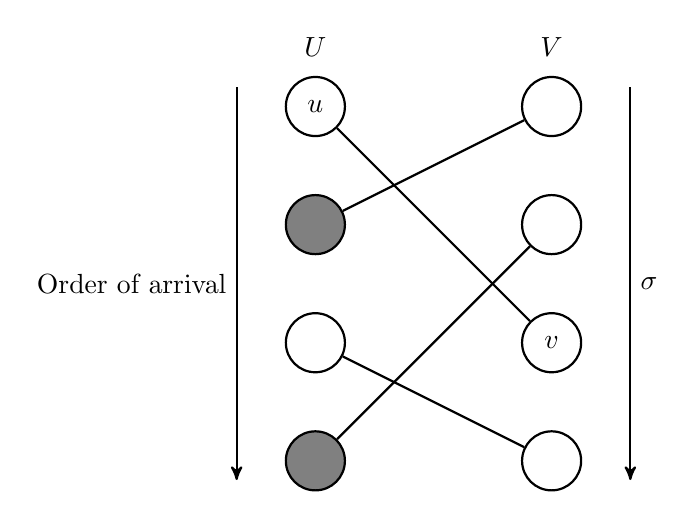
\begin{tikzpicture}[,>=stealth',auto,
  thick,main node/.style={circle,draw, minimum size = 0.75cm}, filled/.style={circle, draw, minimum size = 0.75cm, fill = gray}]

\node[draw = white] (a) at (1, 5.25){$U$};
\node[draw = white] (b) at (4, 5.25){$V$};

\node[main node] (u) at (1, 4.5){$u$};
\node[filled] (v) at (1, 3){};
\node[main node] (w) at (1, 1.5){};
\node[filled] (x) at (1, 0){};

\node[main node] (u1) at (4, 4.5){};
\node[main node] (v1) at (4, 3){};
\node[main node] (w1) at (4, 1.5){$v$};
\node[main node] (x1) at (4, 0){};

\node[draw = white] (m) at (5, -0.375){};
\node[draw = white] (n) at (5, 4.875) {};

\node[draw = white] (o) at (0, -0.375){};
\node[draw = white] (p) at (0, 4.875) {};

\path[]


(u) edge node {} (w1)
(v) edge node {} (u1)
(w) edge node {} (x1)
(x) edge node {} (v1)
(n) edge [->] node [right] {$\sigma$} (m)
(p) edge [->] node [left] {Order of arrival} (o);

\end{tikzpicture}
\caption{The optimal matching $m^*$ is shown in the graph above. Let $t = \sigma(v)$. Then the highlighted nodes represent the set $R_t$.}
\label{fig:Rt}
\end{figure}
\end{center}

However, the rigorous, correct proof is more complex. The fact is that
$u$ and $R_{t}$ are not actually independent in the way we set it
up, because both variables are dependent on $t$. Vertex $u$ is dependent
on $t$ since we have that $\sigma(m^{*}(u))=t$ and the vertex set
$R_{t}$ is by definition dependent on $t$. The correct, but far
less intuitive, proof demonstrates how choosing vertices $v$ and
$u$ randomly and independently of $\sigma$ can result in having
the relation that if vertex $v$ is not matched in $m_{\sigma}$,
then $u\in R_{t}$. In this case $u$ is not dependent on $t$ and
therefore $R_{t}$ and $u$ are independent, which correctly proves
the lemma. Again, we encourage interested readers to read the fully correct
proof in \cite{key-2}. 
\end{proof}
Now we can compute the expected competitiveness. It is easy to see
that the expected size of $m_{\sigma}$ is $\sum_{1\le s\le n}p_{s}$.
Since we are assuming that there exists a perfect matching, that means
the expected competitiveness is 
\[
\frac{|m_{\sigma}|}{|m^{*}|}=\frac{1}{n}\sum_{1\le s\le n}p_{s}.
\]
We will lower bound this competitiveness using Lemma \ref{lem:If-we-define}.
Let us define $S_{t}=\sum_{1\le s\le t}p_{s}$ (note that this makes
our expected competitiveness equal to $\frac{S_{n}}{n}$). We can
rewrite Lemma \ref{lem:If-we-define} to 
\[
1-(S_{t}-S_{t-1})\le\frac{1}{n}S_{t},
\]
which can be simplified to 
\[
1+S_{t-1}\le\left(\frac{n+1}{n}\right)S_{t}.
\]
It turns out that $S_{t}$, and by extension also $\frac{S_{n}}{n}$,
is smallest when all of the inequalities are equalities, which can
be solved to give us 
\[
S_{t}=\sum_{1\le s\le t}\left(\frac{n}{n+1}\right)^{s}.
\]
As a result, our expected competitiveness $\frac{S_{n}}{n}$ is lower
bounded by 
\[
\frac{1}{n}\sum_{1\le s\le n}\left(\frac{n}{n+1}\right)^{s}.
\]
After some non-trivial mathematical manipulation, we can discover
that this value is equivalent to 
\[
1-\left(\frac{n}{n+1}\right){}^{n}.
\]
As $n$ approaches infinity, this value converges to $1-\frac{1}{e}$,
thus concluding our proof.

Now that we demonstrated that the expected competitiveness of \textsc{Ranking} is at least $1-\frac{1}{e}$, the question becomes,
``Is it possible do better?'' The following theorem proven in \cite{key-1},
suggest that no, it is not possible.
\begin{thm}
The competitiveness of any online bipartite matching algorithm is
bounded above by $(1-\frac{1}{e})+O(1)$.
\end{thm}


In \cite{key-1}, the authors demonstrate this theorem by proving
that no online algorithm can do better for a particular graph with
exactly one perfect matching in which the first few incoming vertices
from $U$ are adjacent to all or most of the the vertices in $V$,
but the last few incoming vertices from $U$ are only adjacent to
a few or just one of the vertices in $V$. An example of such a graph is shown in Figure ~\ref{fig:bad}. The reason it causes this
bound, after some nontrivial mathematical analysis, is that the first
vertices received from $U$ have many potential vertices to be matched
with from $V$. Thus, it is unlikely that they will be matched with
their optimal matches, which uses up the few potential matches for
the later incoming vertices from $U$ before the algorithm gets to
them.

\begin{center}
\begin{figure}
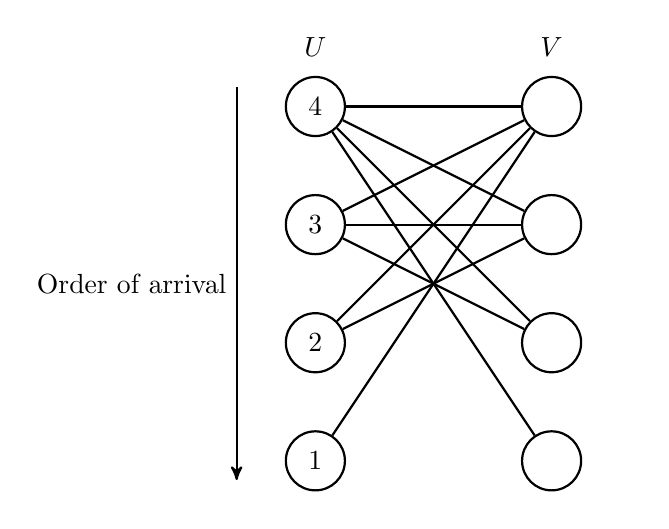
\begin{tikzpicture}[,>=stealth',auto,
  thick,main node/.style={circle,draw, minimum size = 0.75cm}, filled/.style={circle, draw, minimum size = 0.75cm, fill = gray}]

\node[draw = white] (a) at (1, 5.25){$U$};
\node[draw = white] (b) at (4, 5.25){$V$};

\node[main node] (u) at (1, 4.5){4};
\node[main node] (v) at (1, 3){3};
\node[main node] (w) at (1, 1.5){2};
\node[main node] (x) at (1, 0){1};

\node[main node] (u1) at (4, 4.5){};
\node[main node] (v1) at (4, 3){};
\node[main node] (w1) at (4, 1.5){};
\node[main node] (x1) at (4, 0){};

\node[draw = white] (m) at (5, -0.375){};
\node[draw = white] (n) at (5, 4.875) {};

\node[draw = white] (o) at (0, -0.375){};
\node[draw = white] (p) at (0, 4.875) {};

\path[]


(u) edge node {} (u1)
(u) edge node {} (v1)
(u) edge node {} (w1)
(u) edge node {} (x1)

(v) edge node {} (u1)
(v) edge node {} (v1)
(v) edge node {} (w1)

(w) edge node {} (u1)
(w) edge node {} (v1)

(x) edge node {} (u1)

(p) edge [->] node [left] {Order of arrival} (o);

\end{tikzpicture}
\caption{Consider the graph above, where the degree of nodes in $U$ are displayed. Note that unlike in Figure ~\ref{fig:Rt}, the edges in this graph represent $E$ and not a possible matching. Given the order of arrival, it is very unlikely that a randomized algorithm returns the optimal matching.}
\label{fig:bad}
\end{figure}
\end{center}



\section{Online Vertex-Weighted Bipartite Matching}

The online vertex-weighted bipartite matching problem is a generalization of the online bipartite matching problem. The difference is that each vertex in $V$ now has an associated weight. Instead of maximizing the size of the matching, we now aim to maximize the total weight of the vertices of $V$ which are included in the matching. The classic online bipartite matching problem described in Section \ref{section:classic} is the special case where all vertices in $V$ have weight 1.

Formally, the input to the problem is a bipartite graph $G = (U, V, E, \{w_v\}_{v \in V})$. Similarly to before, the vertices in $V$ as well as their weights are known ahead of time and the vertices in $U$ arrive online. The edges of a vertex $u \in U$ are revealed when $u$ arrives. When a vertex arrives it can either be permanently matched to an unmatched neighbor in $V$ or not matched. We aim to maximize the sum of weights of all the matched vertices in $V$. As before, we will assume that $|U| = |V|=n$ and that $G$ contains a perfect matching.

In this section, we will present two algorithms to solve the online vertex-weighted bipartite matching problem. We will then show that these algorithms are generalizations of the algorithms from Section 2, and furthermore that they are able to achieve the same competitive ratios.

\subsection{Generalized Greedy Algorithm}

The obvious greedy solution to this problem is to match a vertex $u \in U$ to its neighbor of greatest weight, or leave it unmatched if it has no remaining neighbors. Call this algorithm $\textsc{Weighted-Greedy}$.

\begin{thm}
\textsc{Weighted-Greedy} is a (1/2)-competitive algorithm for vertex-weighted bipartite matching. Furthermore, this is the best competitive ratio the algorithm can achieve.
\end{thm}

\begin{proof}

First we show that \textsc{Weighted-Greedy} has a competitive ratio of at least 1/2. Let $m$ be the matching produced by \textsc{Weighted-Greedy}. Let $S \subset V$ be the set of vertices which are not matched in $m$. Since $m^*$ is a perfect matching, we have that $|m| + |S| = |m^*|$, where $|m|$ denotes the sum of the weights of all weighted vertices matched in $m$.

Consider a vertex $v \in S$ and $u \in U$ such that $u$ and $v$ are matched in $m^*$. By the same reasoning as in the proof of Lemma~\ref{lem:For-every-vertex}, $u$ must be matched in $m$ to a vertex $v'$ of weight at least $w_v$. But then for each vertex in $S$, there is a vertex in $m$ with at least equal weight. Therefore, $|S| \leq |m|$. It follows that $|m| \geq |m^*|/2$. 

To see that this is the tightest competitive ratio for this algorithm, we offer an example. Consider the following graph.

\begin{center}
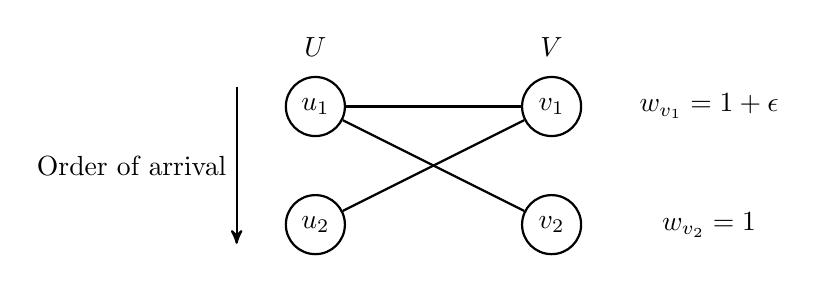
\begin{tikzpicture}[-,>=stealth',auto,
  thick,main node/.style={circle,draw, minimum size = 0.75cm}]

\node[draw = white] (a) at (1, 2.25){$U$};
\node[draw = white] (b) at (4, 2.25){$V$};

\node[main node] (v) at (1, 1.5){$u_1$};
\node[main node] (w) at (1, 0){$u_2$};

\node[main node] (v1) at (4, 1.5){$v_1$};
\node[main node] (w1) at (4, 0){$v_2$};

\node[draw = white] (o) at (0, -0.375){};
\node[draw = white] (p) at (0, 1.875) {};

\node[draw = white] (m) at (6, 0) {$w_{v_2} = 1$};
\node[draw = white] (n) at (6, 1.5) {$w_{v_1} = 1 + \epsilon$};


\path[]


(w) edge node [below] {} (v1)
(v) edge node [below] {} (w1)
(v) edge node [below] {} (v1)
(p) edge [->] node [left] {Order of arrival} (o);

\end{tikzpicture}
\end{center}

Say that vertices arrive in the order $(v_1, v_2)$, and let $w_{v_1} = 1 + \epsilon$ for some $\epsilon > 0$ and $w_{v_2} = 1$. Then the greedy algorithm will match only $(u_1, v_1)$, and the optimal solution will match $(u_1, v_2), (u_2, v_1)$. As $\epsilon$ approaches 0, the competitive ratio approaches $1/2$.

\end{proof}

In Section 2.1 we showed that no deterministic algorithm can have a competitive ratio of better than 1/2 in the unweighted case. Analogously, this is the best competitive ratio that can be achieved by any deterministic algorithm in the weighted case.

\subsection{Generalized Ranking Algorithm}

Consider the algorithm \textsc{Ranking}, as described in Section~\ref{section:ranking}. For an input in which the range of weights is small, this algorithm will perform well. This is reflected in the fact that \textsc{Ranking} is optimal in the case where all weights are equal. However, it turns out that when the range of weights is large, this algorithm can perform very poorly.

We want to generalize \textsc{Ranking} in order to account for the weighted case. We will present a new algorithm which we will call \textsc{Perturbed-Greedy}, and then we will show that this algorithm is equivalent to \textsc{Ranking} in the case where all weights are equal. This algorithm will begin by `perturbing' each of the weights of the vertices in $V$. Then it will follow the \textsc{Greedy} scheme as outlined above.

More formally, the \textsc{Perturbed-Greedy} algorithm will use the function
\[\psi(x) = 1 - e^{x - 1}.\]
The algorithm begins with an initialization step in which we `perturb' the weight of each $v \in V$. To do so, for each $v$ we choose $x$ uniformly at random from $[0, 1]$, and then change the weight of the vertex to $w_v \psi(x)$. Then, for arriving $u \in U$, we match $u$ to the unmatched neighbor with greatest `perturbed' weight, breaking ties by vertex ID.

%\begin{enumerate}
%\item For each $v \in V$, choose $x$ uniformly at random from $[0, 1]$.
%\item For arriving $u \in U$, match $u$ to the unmatched neighbor $v$ with highest value $w_v\psi(x)$.
%\item Break ties by vertex ID.
%\end{enumerate}

Consider the case where all weights are equal. Since $x$ is chosen uniformly at random, choosing vertices according to the highest values of $w_v\psi(x)$ is equivalent to choosing a random ranking. Thus, \textsc{Perturbed-Greedy} is equivalent to \textsc{Ranking} when all weights are equal, as desired.

\begin{thm}
\textsc{Perturbed-Greedy} achieves an approximation ratio of $1 - \frac{1}{e}$ for the vertex-weighted online bipartite matching problem.
\end{thm}

We will offer some intuition as to why the \textsc{Perturbed-Greedy} algorithm is an effective solution to the weighted vertex problem. Consider two previous algorithms which we could use to solve this problem:  \textsc{Weighted-Greedy} and \textsc{Ranking}. When $V$ has a large range of weights, \textsc{Weighted-Greedy} will perform quite well, because the algorithm will place higher priority on matching the larger weights, and the smaller weights matter less when the range is large. On the other hand, we have already noted that \textsc{Ranking} performs well on graphs where the range of weights is small.

To develop a good algorithm for the weighted case, we need something which combines the benefits of each of these algorithms. When weights are highly variable, perturbing the weights will have little effect on their relative ordering. Thus \textsc{Perturbed-Greedy} will behave very similarly to $\textsc{Weighted-Greedy}$, and therefore is able to find a good solution in that case. When weights are very similar, \textsc{Perturbed-Greedy} will behave very similarly to \textsc{Ranking}, and thus does well in this situation as well.

While we will not offer a full proof of the theorem here, we note that this results is consistent with the competitive ratio of \textsc{Ranking}. It turns out that, as is the case with \textsc{Ranking}, this is the optimal competitive ratio for this problem. This result seems reasonable because we know that this is the optimal competitive ratio for the more specific version of this problem.

The proof of the approximation ratio of \textsc{Perturbed-Greedy} is quite similar to the proof of the approximation ratio of \textsc{Ranking} in Section~\ref{section:ranking}. We encourage readers to read this proof in \cite{key-3}.


\section{Stochastic Online Bipartite Matching}

Another interesting variant of the online bipartite matching problem is online bipartite matching with stochastic rewards, as presented in \cite{key-4}. The setup is similar to the classic problem presented in Section 2. As before, the goal is to maximize the number of matchings between a set of $U$ of vertices which are received online and a set $V$ which is known from the start. The difference here is that each matching has some probability of success $p_{uv}$. The algorithms presented in this section are adaptive meaning they immediately learn the result of an attempted matching. The goal is now to maximize the expected number of successful matchings given that some attempts may fail.

This variant of the classic problem was motivated by its practical applications to internet advertising and crowdsourcing. Internet advertising involves matching advertisers' ads to be shown to users of a service where advertisers pay each time a user clicks on an ad (pay-per-click advertising). The likelihood that a user $v$ clicks on an ad $u$ can be modeled by a probability $p_{uv}$. Thus, this matching problem can be modeled as an online stochastic reward matching problem where the service wants to maximize its revenue given a stream of ads to be matched with users. This setup can also model crowdsourcing where each worker $v$ has a probability $p_{uv}$ of completing task $u$ so the online assignment hopes to maximize the expected number of completed tasks.

Solving this problem for arbitrary $p_{uv}$ is an open problem; however \cite{key-4} presents online algorithms and analysis for the problem when all edges have the same probability of success. Formally, for all $u \in U$ and $v \in V$, we have $p_{uv} = p$. These algorithms and their bounds on competitive ratios are still practically usable for the above applications if the variance in values of $p_{uv}$ is small. For example, in online advertising, the probability of a user clicking on an ad is small for almost all users, so using one estimate for $p$ should still give informative, approximate bounds. 

%This special case where $p \rightarrow 0$ is called a vanishing probability and is interesting theoretically on its own. 

\subsection{Stochastic Optimal Algorithm}

As with any online algorithm problem, algorithms are compared to an optimal offline algorithm. A complication here is the non-determinism of the matching success. To mend this, we say that the optimal algorithm is being able to fractionally match vertices. Let $0 \leq x_{uv} \leq 1$ be the fraction of $u$ and $v$ that are matched.  Thus, it aims to maximize the expected number of matchings, given by
\[\sum_{u \in U}{\sum_{v \in V}{p \cdot x_{uv}}},\]
such that no vertex has more than a total of one full matching (i.e., $\sum_{u \in U}{x_{uv}} \leq 1$ for all $u \in U$ and $\sum_{v \in V} x_{uv} \leq 1$ for all $v \in V$). By giving the optimal algorithm more power, we are able to upper bound the best matching of any algorithm.

%\subsection{Adaptive versus Non-Adaptive Algorithms}
%
%The non-determinism of matching success also introduces two classes of algorithms not seen previously in the paper: adaptive and non-adaptive. After each pair is matched, the match's success is immediately computed according to $p$. If successful, $u$ and $v$ are both removed from the set of unmatched vertices. Otherwise, $u$ is permanently left unmatched and $v$ remains free to be matched later.
%
%An adaptive algorithm can learn the result of a matching immediately and attempt to rematch $v$ with a later $u$ if prior matches failed. However, a non-adaptive algorithm does not learn this information until after the algorithm completes. As a result, it may try to rematch a $v$ that was already successfully matched. In this case, each $v$ is only matched to one vertex.
%
%$Explained via the advertising application, a non-adaptive algorithm won't learn if a user clicked on an ad until all ads are assigned, but an adaptive algorithm learns relatively quickly if the user clicked on an ad so it can target future ads to other users. Intuitively, non-adaptive algorithms are less powerful than adaptive algorithms because they learn less information which results in a lower expected number of matches. For a vanishing probability, the competitive ratio for non-adaptive algorithms is at most $1/2$ for both deterministic and randomized algorithms, making them less interesting than their adaptive counterparts.
%
%\begin{thm}
%\label{thm:Non-adaptive}
%For a vanishing probability, any non-adaptive algorithm (deterministic or randomized) achieves a competitive ratio of at most $1/2$ for the stochastic online bipartite matching problem.
%\end{thm}
%\begin{proof}
%The proof finds a particularly bad distribution of inputs for a deterministic algorithm. By Yao's minimax principle, this then bounds the best performance of any randomized algorithm. This bad input distribution is composed of $n$ known $V$ vertices called $v_1, v_2, ..., v_n$ permuted randomly when given to the algorithm. $U$ contains $n/p$ incoming vertices that are seperated into $n$ groups that each contain $1/p$ vertices. These groups arrive in order $U_1, U_2, ..., U_n$, but the sequence of $u$ within each group is permuted randomly. Finally, each group $U_i$ has matching edges to each $v_j$ where $i \leq j \leq n$ with probability $p$ of success. 
%
%The optimal offline algorithm is able to fractionally assign each group $U_i$ to $v_i$ without uncertainty giving $n$ total matchings. Note that a deterministic, non-adaptive algorithm could not follow a similar strategy of matching $U_i$ with $v_i$ because the permutation of $V$ prevents the algorithm from learning the index $i$ for a vertex $u$ until its corresponding $V_i$ has been entirely processed. Additionally, no more $U_j$ groups where $j > i$ have edges to $v_i$ preventing it from obtaining additional potential matches. 
%
%Recall that the probability of at least 1 of $t$ maches is successful is $Pr[t] = 1- (1- p)^t$. The concavity of this function for a fixed $p$ implies that the expected sum of these is maximized when the potential matchings are distributed as evenly as possible. Because the algorithm doesn't learn the indicies of $v$ until it's too late it can be shown that on expectation, the most even assignment is upper bounded by a fractional assignment of each group $U_i$ to all the $v_j$ it has edges with. 
%
%For $v_i$, the number of assignments is $t = \sum_{j=0}^{i-1}{\frac{1}{p(n-j)}}$ \\
%The probability of at least 1 success as $p \rightarrow 0$ is $(1- e^{\sum_{j=0}^{i-1}{\frac{1}{n-j}}})$ \\
%The expected total number of successful matchings $S_n = \sum_{i=1}^n{(1- e^{\sum_{j=0}^{i-1}{\frac{1}{n-j}}})}$\\
%$\lim_{n \rightarrow \infty}{S_n} = 1/2$.
%\end{proof}
%
%Adaptive algorithms have more power than non-adaptive algorithms and are able to achieve better competitive ratios than $1/2$.

Two algorithms are known to perform well for Stochastic Online Bipartite Matching \cite{key-4}. An extension of \textsc{Ranking}, as described in Section~\ref{section:ranking}, called \textsc{Stochastic-Ranking}, performs better when $p \rightarrow 1$. Interestingly enough, a deterministic algorithm, called \textsc{Stochastic-Balance}, performs better when $p \rightarrow 0$. These algorithms will be discussed in more detail in the following sections.

\subsection{Proof Techniques}
The competitive ratio of both of these algorithms is proved using a technique called factor-revealing linear programming \cite{key-5}. Drawing from ideas involving the duality between the algorithm and an adversary, it formulates the adversary's `choice' of some outcomes of the algorithm to maximize the number of vertices that are not matched. The adversary's moves however are constrained to be consistent with the applied algorithm. 

After finding this primal linear program, taking the dual and applying weak duality to some feasible solution of the dual gives an upper bound on the maximum primal objective value, in this case the expected number of failed matchings. Thus, the result is an upper bound of the worst possible performance of the algorithm giving the bound on the competitive ratio. The goal of the algorithmist is to find a set of constraints on the outcomes that follow from running the algorithm and limit the ability of the adversary to maximize the worst case performance. These contraints are not usually nice looking or have obvious intuitive meaning, but with more discoverd constraints, the bound on the competitive ratio will be tighter. This technique is particularly effective in online algorithms because the algorithms' simplicity allows them to be encoded into these constraints. 

\subsection{Stochastic Balance Algorithm}

\textsc{Stochastic-Balance} does not involve any randomization. On an incoming $u$, the algorithm attempts to balance the number of failed attempted matchings among vertices in $V$. To do so, \textsc{Stochastic-Balance} always matches $u$ to the unsuccessfully matched neighbor with the least number of failed matchings. The intuition for why this is effective for $p \rightarrow 0$ is that the concavity of the function for the expected number of matchings when $p \rightarrow 0$ is such that it is maximized when the number of attempts is distributed as evenly as possible.

The analysis of the competitive ratio is made possible by formulating this problem using bin packing. The idea is that each $v$ randomly chooses a bin size $b_v$ that is unknown to the algorithm before the algorithm starts. Each potential matching with $v$ is an item with size $p$ that is placed into the bin for $v$ and adds a load of $p$. We say that $v$ is successfully matched if and only if its bin is full. At that point, it no longer accepts potential matches. In essence, $b_v$ encodes the number of matching attempts needed before a success. This language allows us to easily represent the number of matching attempts as the current load divided by $p$. By linearity of expectation, the expected load on a vertex is equal to the probability of a successful matching.

\begin{defn}Let $b_v$ be a geometric random variable with parameter $p$. It represents the bin size for vertex $v$. 
\[Pr[b_v = pt] = p(1-p)^{t-1}\]
\end{defn}

The factor-revealing linear program of \cite{key-4} defines $f_v(x)$ to be the variables of the linear program corresponding to the probability that vertex $v$ has failed to be matched at the end of the algorithm with resultant load $x$. Note that the number of load levels is linear with $|U|$ because there are at most $|U|$ matching edges to any $v$ which contribute $p$ to the load. The expected number of failures for the algorithm is 
\[\sum_{v}{\sum_{x}f_v(x)},\]
which the adversary attempts to maximize under the constraints of \textsc{Stochastic-Balance}. Finally, $L^*_v$ is an additional variable encoding the load assigned to $v$ by the optimal offline algorithm at the end of the algorithm.

Next, we display the factor-revealing linear program for \textsc{Stochastic-Balance}.

\begin{defn} \textsc{Stochastic-Balance} Factor-Revealing Linear Program \\
\begin{alignat}{3}
\text{maximize}  \quad & \sum_{x}{\sum_{v}f_v(x)} & \nonumber \\
\text{subject to} \quad & \sum_x{\sum_v{f_v(x)(1-p)^{-x/p}}} = n & \\
& \sum_{y \leq x}{\sum_v{(1+L^*_u)f_u(y)}} + (1-p)^{x/p}\sum_{y>x}{(1-p)^{-y/p}\left (\sum_u{f_y(y)}\right )} \leq n & \quad \forall{x} \\
& \sum_v{((1-p)^{-L^*_v/p} + \sum_{y<L^*_v}{f_v(y)(1 + L^*_v - x)(1-p)^{-y/p})}} \leq n & \quad \forall{x}
\end{alignat}
\label{defn:lp}
\end{defn}

We will prove the correctness of constraints 4.1 and 4.2 to give a flavor for how these constraints are discovered. The full proof of the derivation of constraint 4.3 is quite involved, but interested readers can see it in \cite{key-4}. Before proceeding, we give the following definitions.

\begin{defn}Let $L^{\infty}_v(b)$ be the load on vertex $v$ given that $b$ is modified such that $b_v = \infty$ but $b_{v'}$ for $v \neq v'$ is the same. In words, it is the load on $v$ after the algorithm runs with an unlimited threshold for $v$ making it not possible to be successfully matched. 
\end{defn}

\begin{defn}
Let $q_v(x)$ be the probability that $x$ is the resulting load for $v$ after any run of the algorithm. This is computed by summing the probabilities of randomly obtaining each $b$ that gives load $x$ for $v$. Formally, we have
\[q_v(x) = \sum_{b: L^{\infty}_v(b)=x}\left ({\prod_{z \neq v}{Pr[b_z]}} \right).\]
\end{defn}

We are now equipped to prove the correctness of the constraints 4.1 and 4.2. We will do so through the following Lemmas.

\begin{lem} $f_v(x) = (1-p)^{(x/p)}q_v(x)$ 
\begin{proof}
\[f_v(x) = Pr[(b_v > x) \wedge (L^{\infty}_u(b_v) = x)]\] 
\[f_v(x) = Pr[b_v > x]Pr[L^{\infty}_u(b_v) = x]\] 
\[f_v(x) = (1-p)^{(x/p)}q_v(x)\] 

This follows from representing the probability of a resulting load being unsuccessful as the intersection of when the load is less than its threshold and the algorithm terminates with $x$. By independence, this separates giving the resulting expression where $(1-p)^{(x/p)}$ indicates that the matching fails $x/p$ times and $q_v(x)$ is probability of the resulting load. We can represent the probability that load $x$ succeeds for vertex $v$ as $g_v(x)$ and find a similar looking expression. 
\end{proof}
\end{lem}

\begin{lem} $g_v(x) = p(1-p)^{(x/p-1)}\sum_{y \geq x}{q_v(y)}$ 
\begin{proof}
\[g_v(x) = Pr[(b_v = x) \wedge (L^{\infty}_v(b_v) \geq x)]\]
\[g_v(x) = Pr[b_v = x]Pr[L^{\infty}_v(b_v) \geq x]\]
\[g_v(x) = p(1-p)^{(x/p-1)}\sum_{y \geq x}{q_v(y)}\] 

This follows from noting that a load is successful if it equals its threshold. But also, the resulting load of the algorithm if there is no limit on the load must give some load greater than $x$ or $x$ is not possibly obtained. This probability of the first part is $ p(1-p)^{(x/p-1)}$ while the probability of the second is the sum of each of these disjoint $q_v(y)$ events.
\end{proof}
\end{lem}

\begin{lem} Constraint 4.1: $\sum_x{\sum_v{f_v(x)(1-p)^{-x/p}}} = n$
\begin{proof}
 Because $f_v(x)$ and $g_v(x)$ are defined complementarily, the sum over the possible loads and vertices must equal the total number of vertices, $\sum_v{\sum_x{(f_v(x) + g_v(x))}} = n$. Substituting $g_v(x)$ for $f_v(x)$ gives Constraint 4.1.
\end{proof}
\end{lem}

\begin{lem} Constraint 4.2: $\sum_{y \leq x}{\sum_v{(1+L^*_u)f_u(y)}} + (1-p)^{x/p}\sum_{y>x}{(1-p)^{-y/p}(\sum_u{f_y(y)})} \leq n$
\begin{proof}
\[\sum_{y \leq x}{\sum_v{L^*_vf_v(y)}} \leq \sum_{y \leq x}{y \sum_v{(f_v(y) + g_v(y))}} + x\sum_{y > x}{\sum_v{(f_v(y) + g_v(y))}}\]
\[\sum_{y \leq x}{\sum_v{(1+L^*_v)f_v(y)}} + (1-p)^{x/p}\sum_{y>x}{(1-p)^{-y/p}(\sum_v{f_y(y)})}
\leq \sum_x{\sum_v{f_v(x)(1-p)^{-x/p}}} = n\]

This is because for a vertex $v$ that ends up with load $x$, all $v'$ on the optimal offline solution that took a possible matching from $v$ must have had a lower load at the time to be picked before $u$ by \textsc{Stochastic-Balance}. So the expected sum of optimal loads assigned when the algorithm fails an assignment is less than the sum of expected load of the failed vertices produced by  \textsc{Stochastic-Balance}. Substituting $g_v(x)$ for $f_v(x)$, simplifying, and appling the equality learned in Constraint 4.1 gives Constraint 4.2.
\end{proof}
\end{lem}

Using this linear program, \cite{key-4} proves the following theorem.

\begin{thm} \textsc{Stochastic-Balance} achieves a competitive ratio for the stochastic online bipartite matching problem of
\[\frac{1+(1-p)^ {2/p}}{2}\]
\end{thm}

By taking the dual of this linear program given in Definition~\ref{defn:lp}, finding a feasible solution, and applying weak duality, \cite{key-4} was able to to obtain an upper bound on the number of failed matchings which \textsc{Stochastic-Balance} will encounter. The full derivation of the competitive ratio is not given here, but we encourage interested readers to consult \cite{key-4} for the full proof.


\subsection{Stochastic Ranking Algorithm}

\textsc{Stochastic-Ranking} is very similar to \textsc{Ranking}, as described in Section~\ref{section:ranking}. It begins by randomly permuting the set of vertices $V$. Upon an incoming vertex to be matched, the algorithm matches it with the highest ranked neighbor that has not been successfully matched. Unlike our previous proofs for the competitive ratio of \textsc{Ranking}, the proof for \textsc{Stochastic-Ranking} uses a Factor-Revealing Linear Program. We won't go into the details of this linear program, but it compares the difference in performance of \textsc{Stochastic-Ranking} from the optimal offline algorithm by classifying matchings as good matchings or bad matchings. A bad matching occurs when matched edge $(u, v)$ has $\sigma(v) < \sigma(m^*(u))$. Otherwise, a matching is a good matching. The linear program finds constraints relating the load caused by good and bad matchings resulting from the algorithm to prevent the adversary from maximizing the number of failed matchings.

\begin{thm}
\textsc{Stochastic-Ranking} achieves a competitive ratio for the stochastic online bipartite matching problem of
\[\left (1-\frac{1}{e} \right ) - \left (1-\frac{2}{e}\right ) \cdot (1-p)^{1/p}\]

\end{thm}

The technique for proving this competitive ratio is very similar to the technique used to prove Theorem 18. We again encourage interested readers to consult the proof in \cite{key-4}.


\subsection{Discussion}

The intersection of the two functions for the competitive ratios of \textsc{Stochastic-Balance} and \textsc{Stochastic-Ranking} shows that the latter performs better when $p < 0.26$. This is illustrated in Figure~\ref{fig:graph}. Thus unlike the classic and weighted cases, a deterministic algorithm not only achieves a better competitive ratio than 1/2 but also so far is known to perform better than the randomized algorithm as $p \rightarrow 0$. Also note that these competitive ratios are consistent with the reduction to the non-stochastic case where $p = 1$. In this case, \textsc{Stochastic-Balance} has a competitive ratio of 1/2 while \textsc{Stochastic-Ranking} has a competitive ratio of $1 - 1/e$.

\begin{figure}
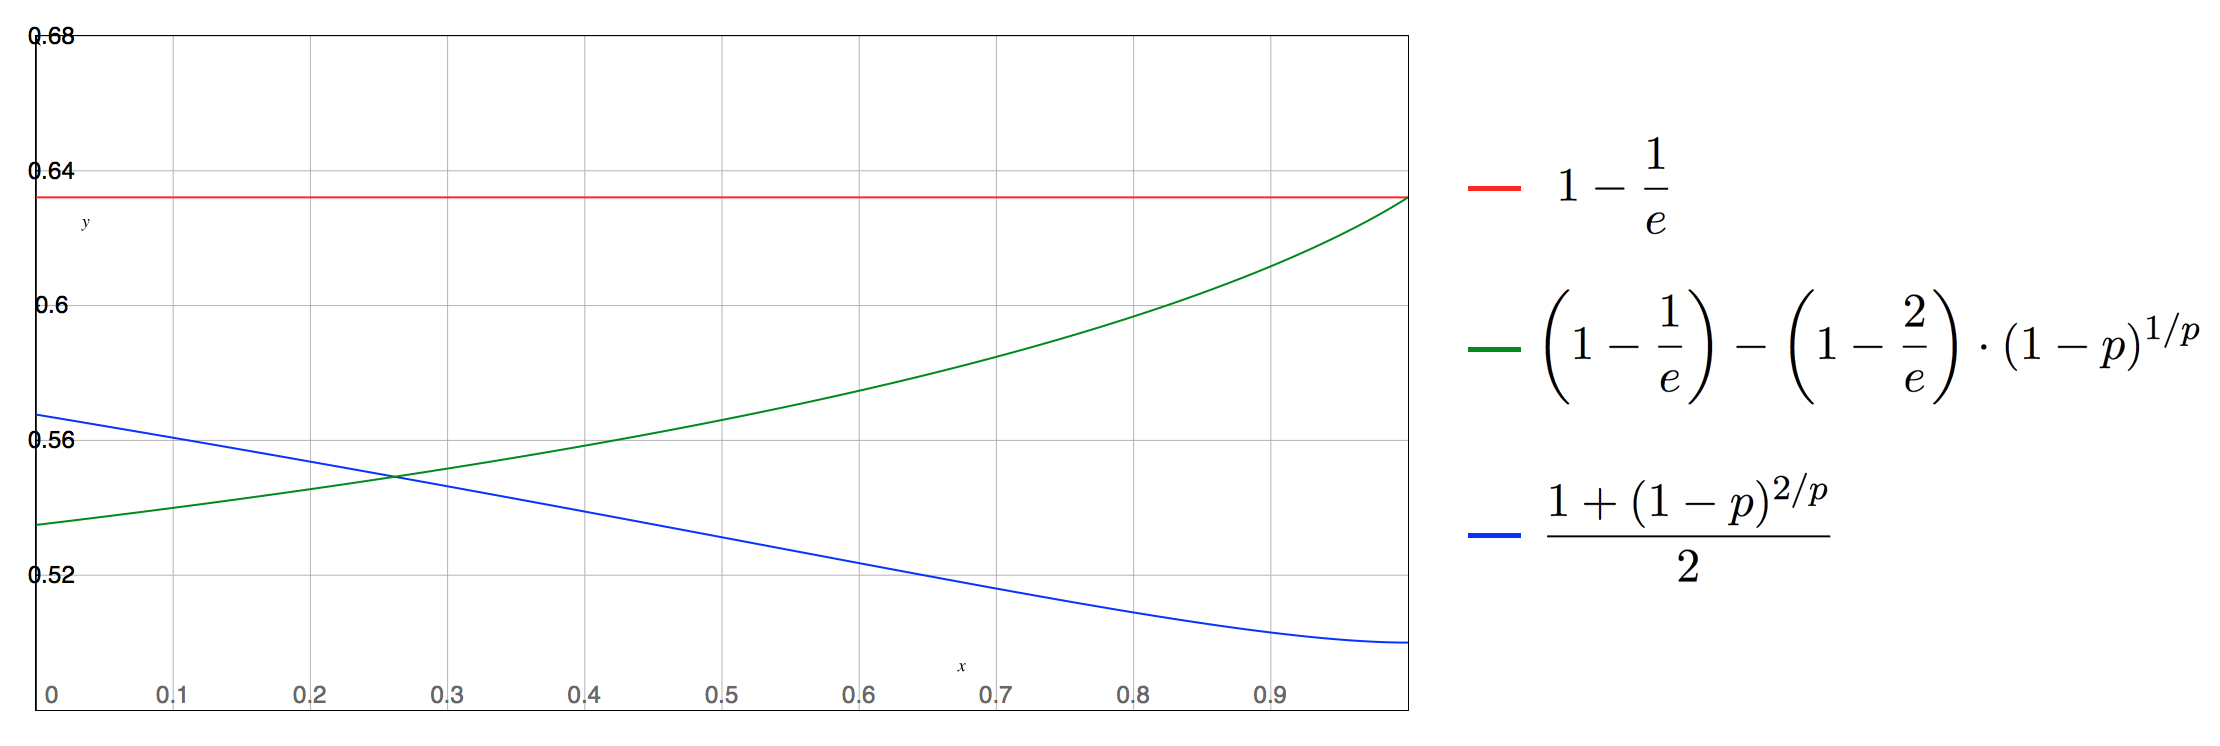
\includegraphics[width=6.5in]{graph.png}
\caption{Shown above are the competitive ratios of \textsc{Ranking} (red), \textsc{Stochastic-Balance} (green), and \textsc{Stochastic-Ranking} (blue).}
\label{fig:graph}
\end{figure}
%\section{Conclusion}

%Since the original paper published in 1990, the online bipartite matching problem and its variants have gained a lot of attention, in particular in regards to its applications to online advertising. Through this paper we explored the original online bipartite matching problem, the problem with weighted vertices, and the problem with stochastic rewards. Without offering complete formal proofs, we have presented many of the most important results pertaining to this set of problems.

\section{Acknowledgements}

We would like to thank Professor Karger for a great semester. We would also like to thank Anvisha Pai, Fermi Ma, and Matt Jordan for their constructive feedback.

\begin{thebibliography}{{[}AGKM{]}}
\bibitem[{[}KVV{]}]{key-1} R. Karp, U. Vazirani, and V. Vazirani,
\textquotedblleft{}An optimal algorithm for online bipartite matching,\textquotedblright{}
in Proceedings of the 22nd Annual ACM Symposium on Theory of Computing,
1990. (http://www.cs.berkeley.edu/\textasciitilde{}vazirani/pubs/online.pdf)

\bibitem[{[}BM{]}]{key-2} B. Birnbaum and C. Mathieu, \textquotedblleft{}Online
bipartite matching made simple,\textquotedblright{} 2008. (http://cs.brown.edu/\textasciitilde{}claire/Publis/sigactnews08.pdf)

\bibitem[{[}GM{]}]{key-19}Gagan Goel and Aranyak Mehta. Online budgeted
matching in random input models with applications to adwords. In SODA
'08: Proceedings of the nineteenth annual ACM-SIAM symposium on discrete
algorithms, pages 982-991, Philadelphia, PA, USA, 2008. Society for
Industrial and Applied Mathematics.

\bibitem[{[}AGKM{]}]{key-3} Gagan Aggarwal, Gagan Goel, Chinmay Karande,
and Aranyak Mehta, \textquotedblleft{}Online vertex-weighted bipartite
matching and single-bid budgeted allocations,\textquotedblright{}
SODA, 2011. (arXiv:1007.1271 {[}cs.DS{]})

\bibitem[{[}MP{]}]{key-4} A. Mehta and D. Panigrahi, \textquotedblleft{}Online
matching with stochastic rewards,\textquotedblright{} FOCS, 2012,
pp. 728-737. (http://www.cs.duke.edu/\textasciitilde{}debmalya/papers/focs12-matching.pdf)

\bibitem[{[}JMMSV{]}]{key-5} K. Jain, M. Mahdian, E. Markakis, A. Saberi, and V. V.
Vazirani, \textquotedblleft{}Greedy facility location algorithms analyzed using
dual fitting with factor-revealing lp,\textquotedblright{} J. ACM, vol. 50, no. 6, pp. 795-824, 2003.

\end{thebibliography}
 

\end{document}
